\documentclass[a4paper,12pt,oneside,openany,table,xcdraw]{article}

\usepackage{setspace}
\usepackage{multirow}
\usepackage{hyperref}
\usepackage{caption}
\usepackage{indentfirst}

\usepackage[brazilian]{babel}
\usepackage[utf8x]{inputenc}
\usepackage{amsmath, graphicx, enumerate}
\usepackage{float, verbatim}
\usepackage[colorinlistoftodos]{todonotes}
\usepackage{makeidx} % Para o sumário
\usepackage{geometry}

\usepackage{mathtools,listings} %%
\usepackage{color} %red, green, blue, yellow, cyan, magenta, black, white
\definecolor{mygreen}{RGB}{28,172,0} % color values Red, Green, Blue
\definecolor{mylilas}{RGB}{170,55,241}

\graphicspath{{img/}}
\geometry{a4paper, hmargin={3cm, 3cm}, vmargin={3cm, 2cm} }
\setlength{\parindent}{1.0cm}
\captionsetup{font=small}

\begin{document}
\newcommand{\thedepartment}{Faculdade de Engenharia Elétrica}
\newcommand{\thecourse}{FEELT}
\newcommand{\thetitle}{LISTA DE EXERCÍCIOS EXTRAS 1}
\newcommand{\thetype}{Relatório da Disciplina de Sinais e Sistemas 2}
\newcommand{\theproftitle}{Doutor em Engenharia Elétrica com ênfase em Telecomunicações}
\newcommand{\thestudent}{Lesly Viviane Montúfar Berrios\\
\centering11811ETE001}
\newcommand{\theadvisor}{Prof. Alan Petrônio Pinheiro}
\newcommand{\thecity}{Uberlândia}

\thispagestyle{empty}\newcommand*{\themonth}{\ifthenelse{\the\month < 2}{Janeiro }
                  {\ifthenelse{\the\month < 3}{Fevereiro }
                  {\ifthenelse{\the\month < 4}{Março }
                  {\ifthenelse{\the\month < 5}{Abril }
                  {\ifthenelse{\the\month < 6}{Maio }
                  {\ifthenelse{\the\month < 7}{Junho }
                  {\ifthenelse{\the\month < 8}{Julho }
                  {\ifthenelse{\the\month < 9}{Agosto }
                  {\ifthenelse{\the\month < 10}{Setembro }
                  {\ifthenelse{\the\month < 11}{Outubro }
                  {\ifthenelse{\the\month < 12}{Novembro }{Dezembro }}}}}}}}}}}}
                  
\begin{titlepage}
\begin{center}

	\vspace{-0.5cm}

  \begin{figure}[hbt!]
		\begin{center}
		   
\includegraphics[width=2.8cm]{ufu-logo.png}
		\end{center}
	\end{figure}
 	%\vspace{-4cm}

%\begin{doublespacing}

  \Large{\textbf{Universidade Federal de Uberlândia}}\\
  \large{\thedepartment}\\
  \large{\thecourse}\\


\vspace{5.8cm}
  \par
  \large\textbf{\thetitle}
\vspace{5.8cm} 

%\end{doublespacing}
  \par
  \thetype\\
  por\\
  %\hspace{2cm}\large{}\\

\vspace{0.8cm}
\par
  \normalsize{\thestudent}\\ [2cm]
  \theadvisor

\par\vfill
  \thecity, \themonth / \the\year

\end{center}

\end{titlepage}

\lstset{language=Matlab,%
    %basicstyle=\color{red},
    breaklines=true,%
    morekeywords={matlab2tikz},
    keywordstyle=\color{blue},%
    morekeywords=[2]{1}, keywordstyle=[2]{\color{black}},
    identifierstyle=\color{black},%
    stringstyle=\color{mylilas},
    commentstyle=\color{mygreen},%
    showstringspaces=false,%without this there will be a symbol in the places where there is a space
    numbers=left,%
    numberstyle={\tiny \color{black}},% size of the numbers
    numbersep=9pt, % this defines how far the numbers are from the text
    emph=[1]{for,end,break},emphstyle=[1]\color{red}, %some words to emphasise
    %emph=[2]{word1,word2}, emphstyle=[2]{style},    
}


%% Comeca o documento !

\onehalfspacing
\tableofcontents % sumário
\newpage

\section{Exercício 1}
Os cálculos são observados abaixo.

\begin{figure}[H]
\centering
\captionsetup{font=scriptsize}
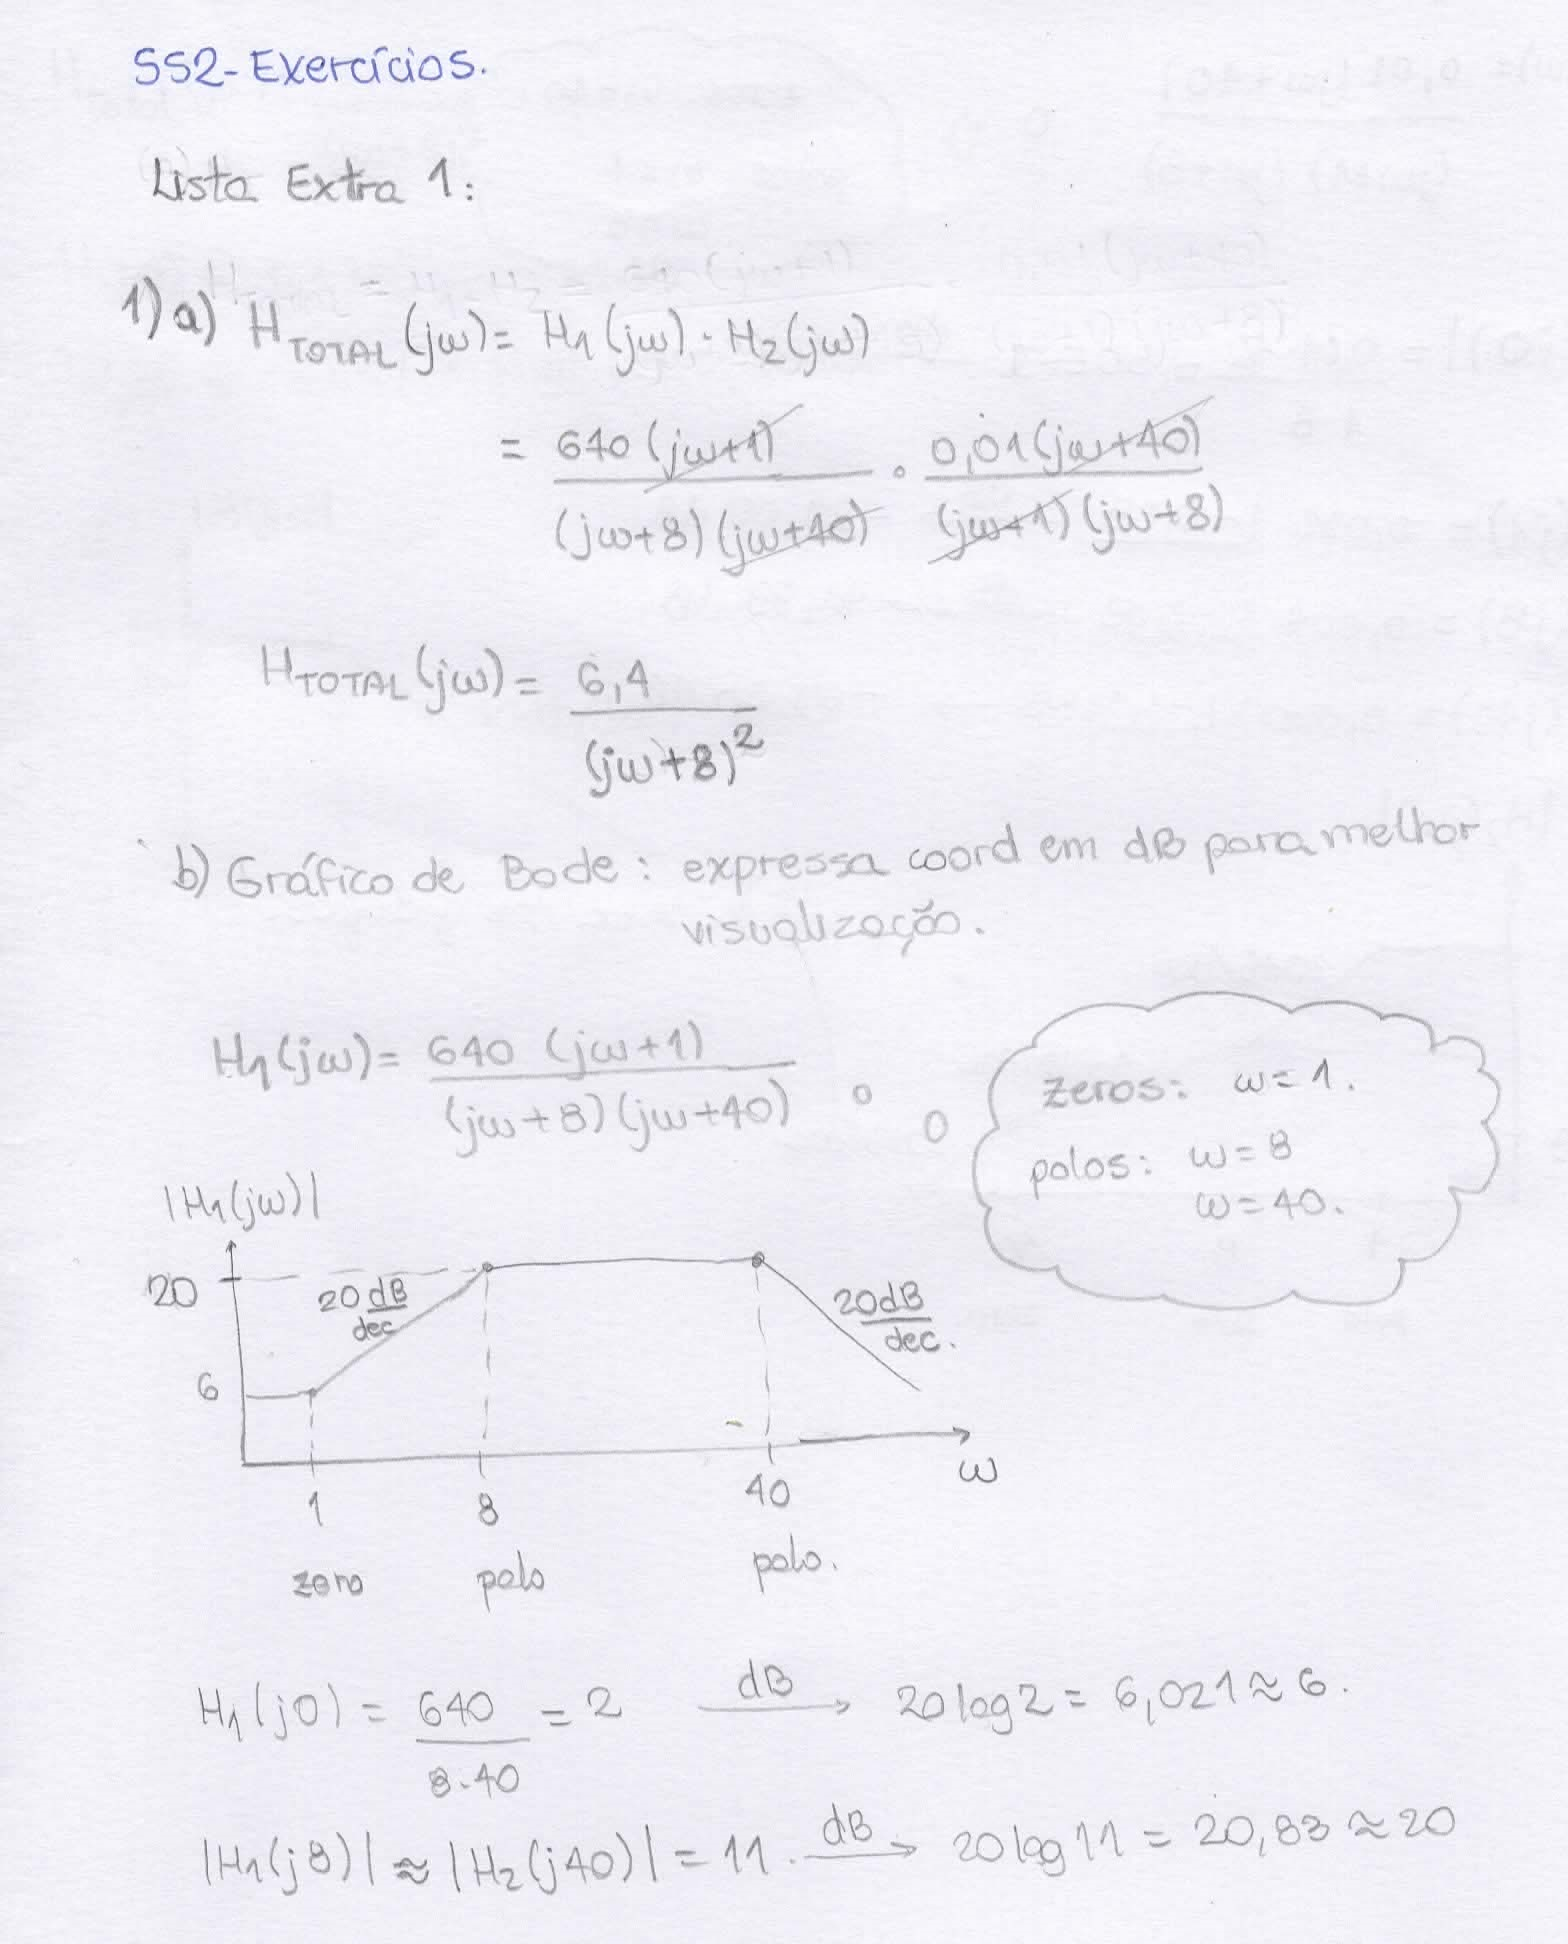
\includegraphics[width=14.5cm]{scan1}
\caption{Resolução do exercício 1.}
\label{scan:1}
\end{figure}

\begin{figure}[H]
\centering
\captionsetup{font=scriptsize}
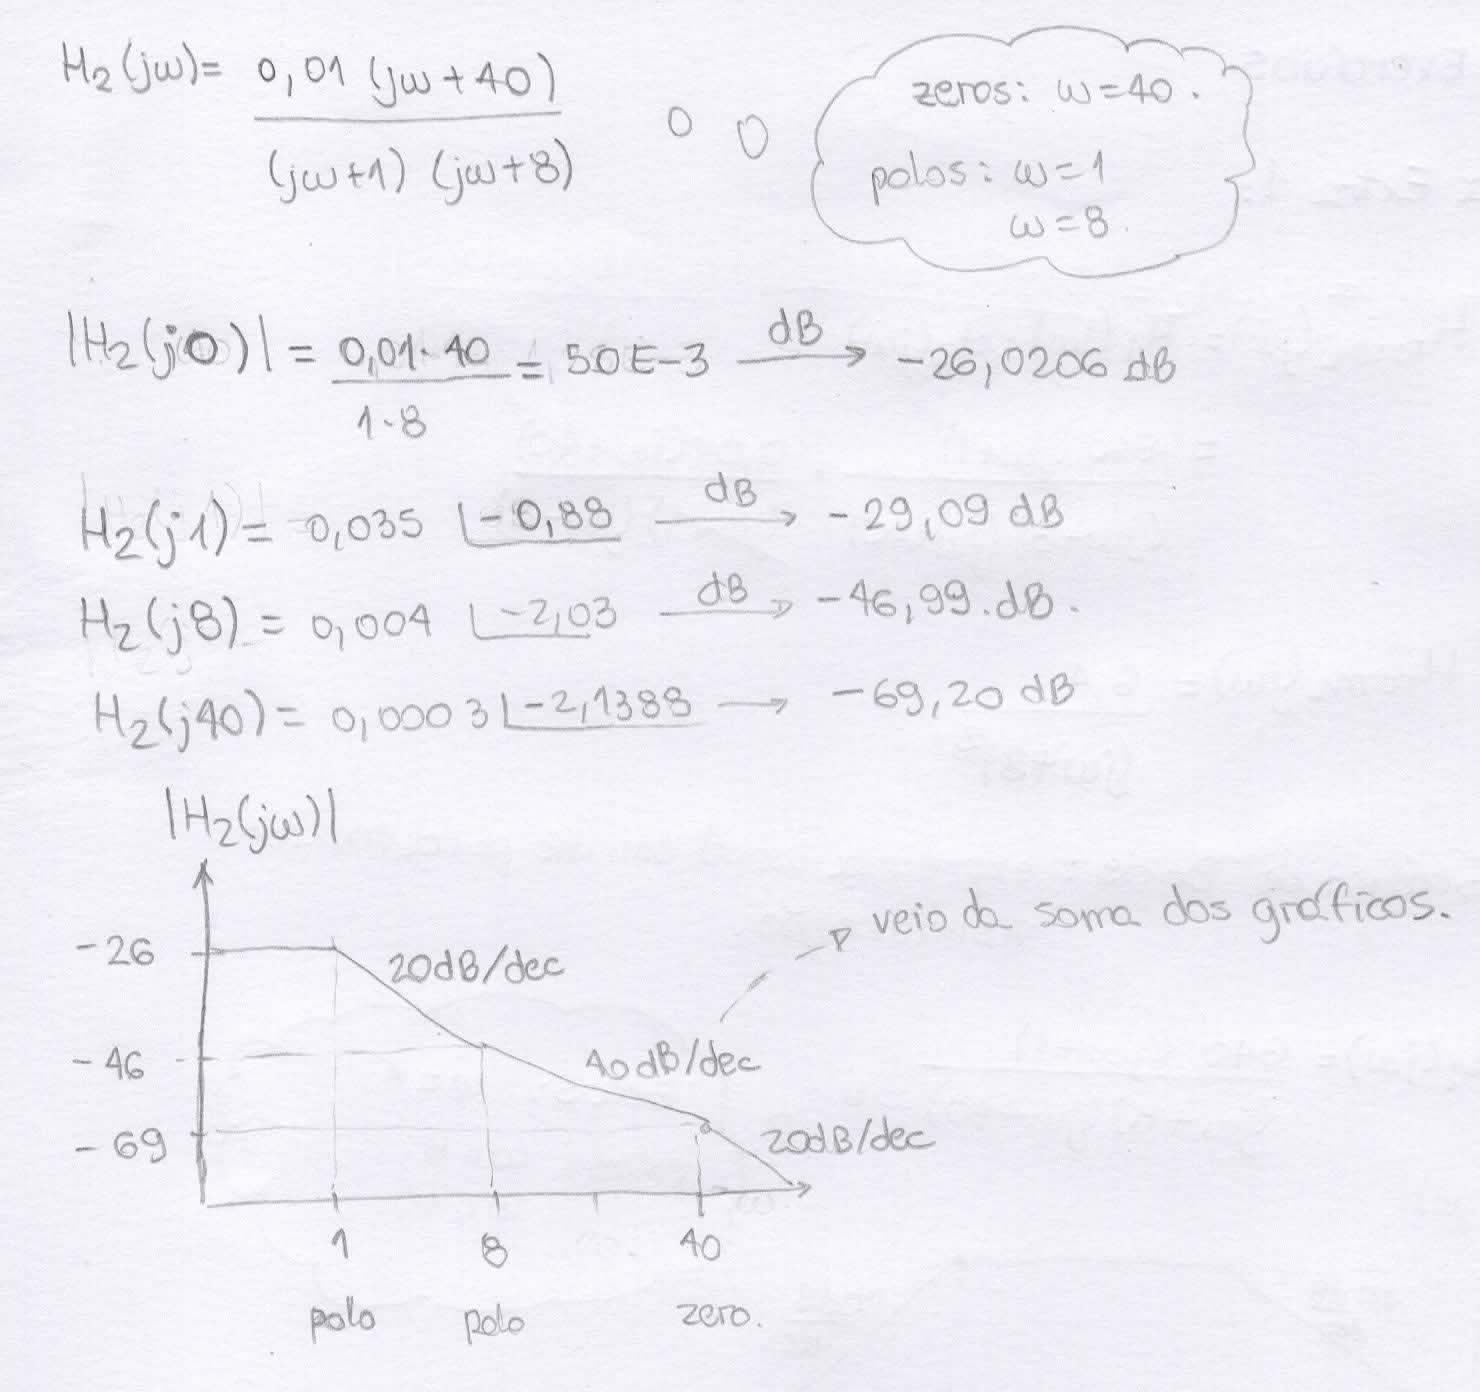
\includegraphics[width=14.5cm]{scan2}
\caption{Resolução do exercício 1.}
\label{scan:1}
\end{figure}

\begin{figure}[H]
\centering
\captionsetup{font=scriptsize}
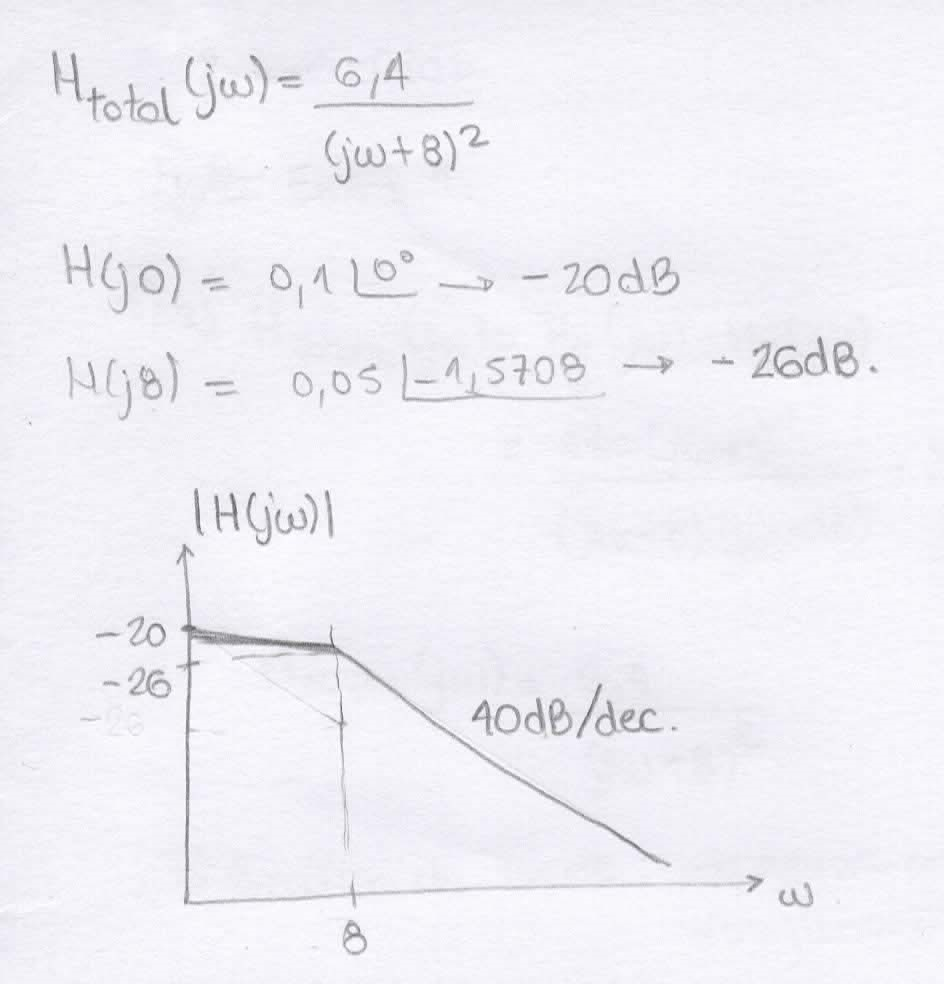
\includegraphics[width=14.5cm]{scan3}
\caption{Resolução do exercício 1.}
\label{scan:1}
\end{figure}

\vspace{1cm}
Para o item (b), utilizou o código abaixo, para assim plotar os gráficos das Figuras \ref{bode:h1}, \ref{bode:h2} e \ref{bode:htotal}. Na escala linear, tem-se os gráficos das Figuras \ref{bode:h1:linear}, \ref{bode:h2:linear} e \ref{bode:htotal:linear}.
\lstinputlisting{../Ex1.m}
\vspace{1cm}

\begin{figure}[H]
\centering
\captionsetup{font=scriptsize}
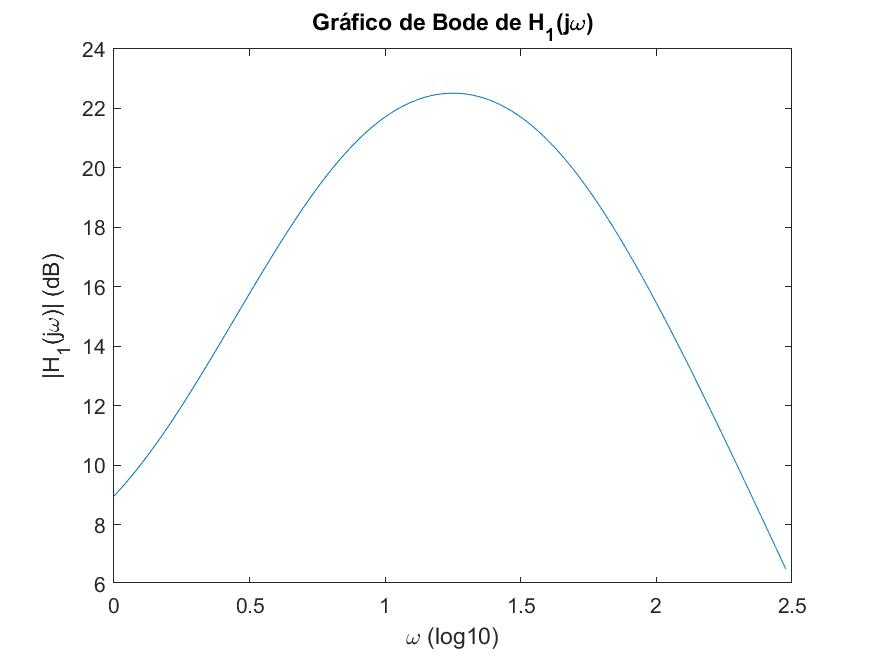
\includegraphics[width=14.5cm]{Ex1_b1}
\caption{Resolução do exercício 1.}
\label{bode:h1}
\end{figure}

\begin{figure}[H]
\centering
\captionsetup{font=scriptsize}
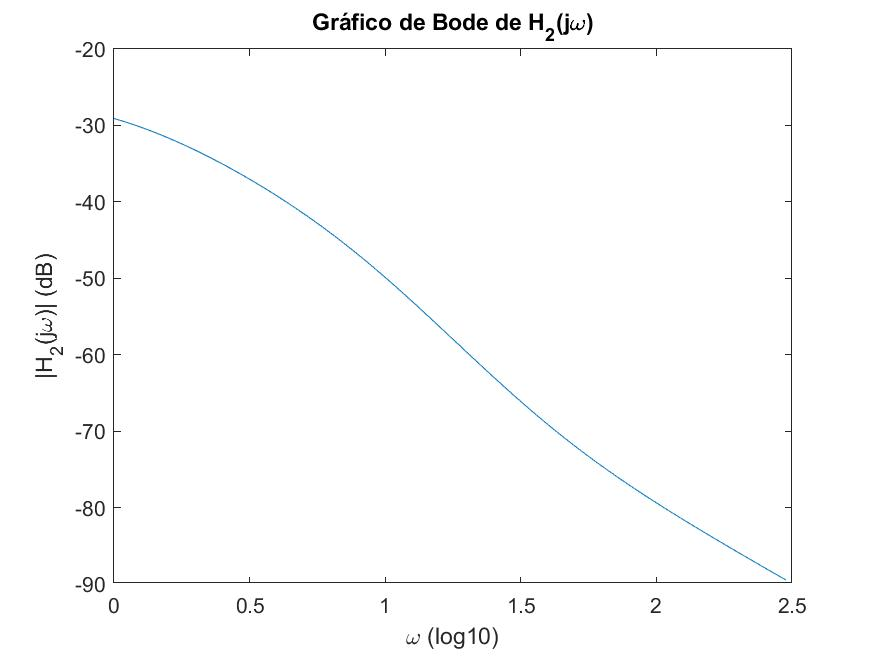
\includegraphics[width=14.5cm]{Ex1_b2}
\caption{Resolução do exercício 1.}
\label{bode:h2}
\end{figure}

\begin{figure}[H]
\centering
\captionsetup{font=scriptsize}
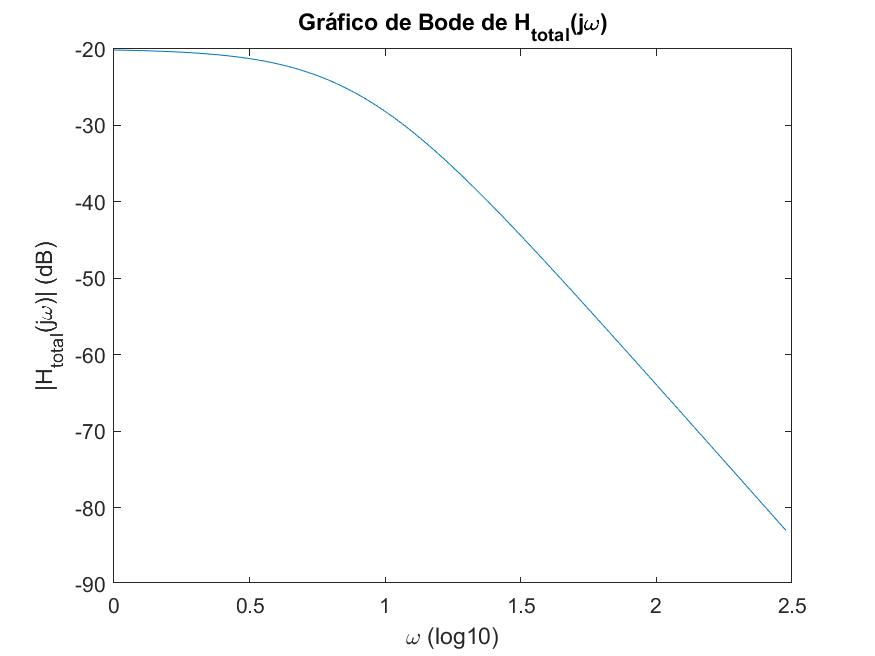
\includegraphics[width=14.5cm]{Ex1_btot}
\caption{Resolução do exercício 1.}
\label{bode:htotal}
\end{figure}
\begin{figure}[H]
\centering
\captionsetup{font=scriptsize}
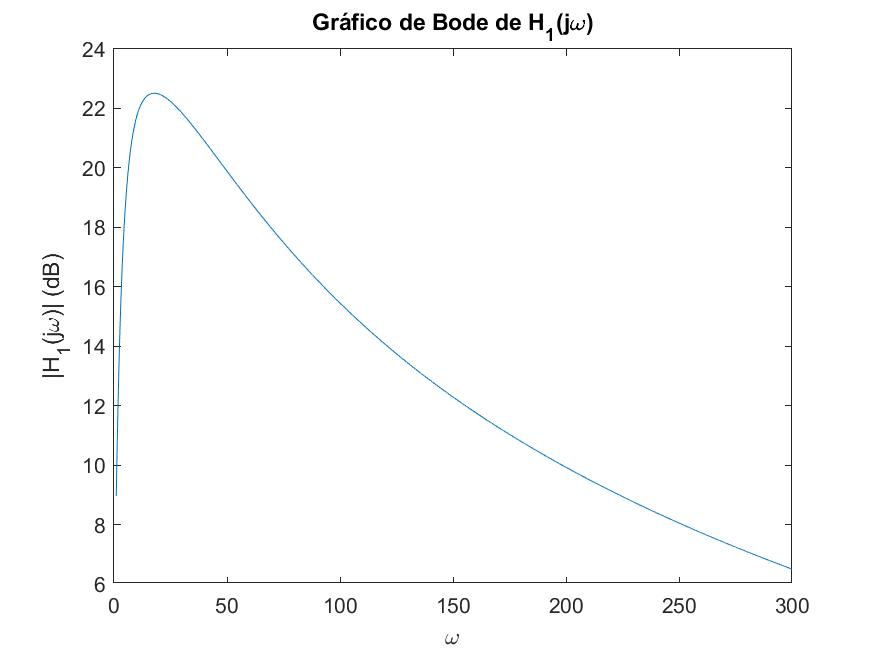
\includegraphics[width=14.5cm]{Ex1_c1}
\caption{Resolução do exercício 1.}
\label{bode:h1:linear}
\end{figure}

\begin{figure}[H]
\centering
\captionsetup{font=scriptsize}
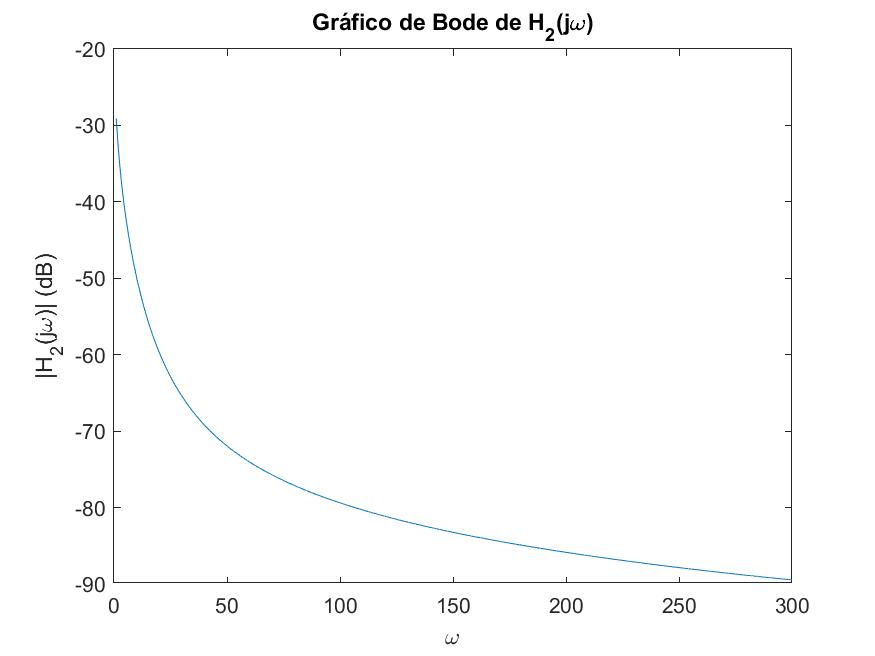
\includegraphics[width=14.5cm]{Ex1_c2}
\caption{Resolução do exercício 1.}
\label{bode:h2:linear}
\end{figure}

\begin{figure}[H]
\centering
\captionsetup{font=scriptsize}
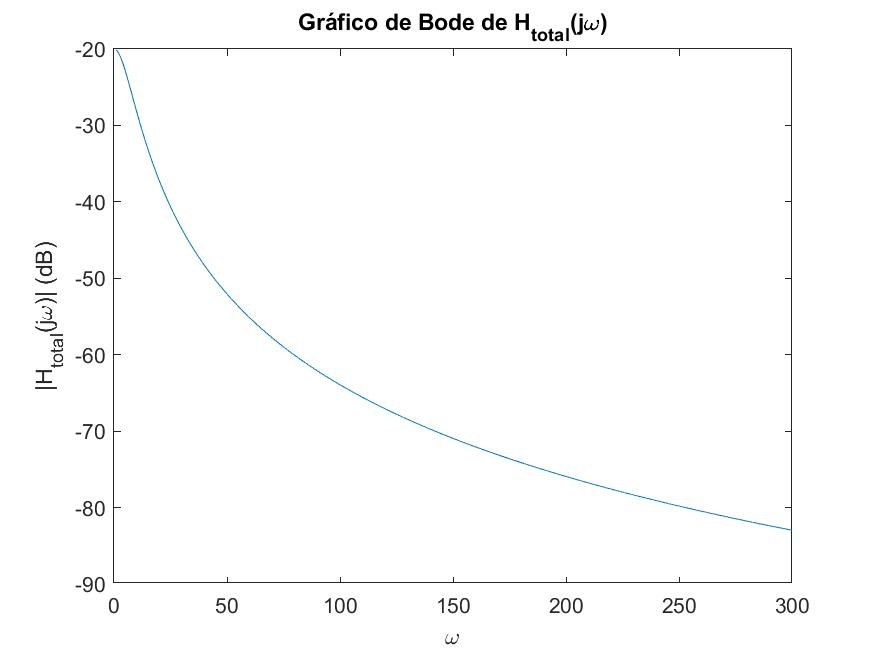
\includegraphics[width=14.5cm]{Ex1_ctot}
\caption{Resolução do exercício 1.}
\label{bode:htotal:linear}
\end{figure}

\vspace{1cm}
Fazendo $\omega=2\pi \cdot f$, para $f=1Hz$ e $f=60Hz$, tem-se respectivamente um ganho de 0.0618486 (atenuação) e $4.50114e-05$ (atenuação).
\lstinputlisting{../polos_zeros.m}
\vspace{1cm}

\section{Exercício 2}




\end{document}